\section{Hedging Interest Rate Risk}
The term structure is given by
\[
R(T)=\beta_1+\beta_2T+\beta_3T^2,\quad (\beta_1,\beta_2,\beta_3)=(0.04,0.012,-0.0015),\qquad
D(T)=e^{-R(T)T}.
\]
The 8-year 6\% semiannual bond (face 100) pays cash flows \(3\) at \(T_k=0.5k\), \(k=1,\dots,15\), and \(103\) at \(T_{16}=8\).

\subsection*{1.1 \quad Bond price}

The price follows from discounting each payment:
$
B_t=\sum_{k=1}^{16}\text{CF}_k\,e^{-R(T_k)T_k}.
$
Representative terms are:

\begin{center}
\begin{tabular}{c c c c c}
$k$ & $T_k$ & $\text{CF}_k$ & $R(T_k)$ & $\text{CF}_k e^{-R(T_k)T_k}$ \\ \hline
1 & 0.5 & 3   & 0.0450 & 2.934 \\
2 & 1.0 & 3   & 0.0505 & 2.854 \\
3 & 1.5 & 3   & 0.0548 & 2.771 \\
\vdots & \vdots & \vdots & \vdots & \vdots \\
14 & 7.0 & 3   & 0.0820 & 2.168 \\
15 & 7.5 & 3   & 0.0829 & 2.134 \\
16 & 8.0 & 103 & 0.0832 & 84.998 \\
\end{tabular}
\end{center}

Summing all discounted flows gives
$
\boxed{B_t \approx 110.858}
$

\subsection*{1.2 \quad Level and curvature factor durations}

Write the curve as
$
R(T)=\beta_1 f_{\text{lev}}(T)+\beta_2 f_{\text{slope}}(T)+\beta_3 f_{\text{curv}}(T),\qquad
f_{\text{lev}}(T)=1,\ f_{\text{curv}}(T)=T^2.
$
For a generic bond:
\[
P=\sum_{k=1}^n\text{CF}_k e^{-R(T_k)T_k},
\]
and the factor duration with respect to factor \(j\) is:
\[
D_j=-\frac{1}{P}\frac{\partial P}{\partial\beta_j}
   =\frac{1}{P}\sum_{k=1}^n\text{CF}_k\,T_k\,f_j(T_k)\,e^{-R(T_k)T_k}.
\]

For the 8-year bond:
\[
D_{\text{lev},B}
=\frac{1}{B_t}\sum_{k=1}^{16}\text{CF}_k T_k e^{-R(T_k)T_k}\approx \boxed{\text{6.619}},\qquad
D_{\text{curv},B}
=\frac{1}{B_t}\sum_{k=1}^{16}\text{CF}_k T_k^3 e^{-R(T_k)T_k}\approx \boxed{\text{380.495}}
\]

A zero maturing at \(T\) has price \(Z_t(T)=100e^{-R(T)T}\) and factor durations
$
D_{\text{lev}}^{z}(T)=T, D_{\text{curv}}^{z}(T)=T^3
$

For the 1-year and 7-year zeros:
\begin{center}
\begin{tabular}{c c c c}
 & $Z_t(T)$ & $D_{\text{lev}}^{z}(T)$ & $D_{\text{curv}}^{z}(T)$ \\ \hline
$T=1$ & $95.075$ & $1$   & $1$ \\
$T=7$ & $70.223$ & $7$   & $343$ \\
\end{tabular}
\end{center}

\subsection*{1.3 \quad Factor-duration hedge}

The hedged portfolio:
$
P_t = B_t + k_1 Z_t(1) + k_7 Z_t(7)
$
has factor–dollar durations:
\[
FD_{\text{lev}}
= B_t D_{\text{lev},B}
+ k_1 Z_t(1) D_{\text{lev}}^{z}(1)
+ k_7 Z_t(7) D_{\text{lev}}^{z}(7),
\]
\[
FD_{\text{curv}}
= B_t D_{\text{curv},B}
+ k_1 Z_t(1) D_{\text{curv}}^{z}(1)
+ k_7 Z_t(7) D_{\text{curv}}^{z}(7).
\]
Setting both exposures to zero yields
\[
\begin{cases}
B_t D_{\text{lev},B} + k_1 Z_t(1) + 7k_7 Z_t(7)=0,\\
B_t D_{\text{curv},B} + k_1 Z_t(1) + 343k_7 Z_t(7)=0.
\end{cases}
\]
Using
$
B_t=110.858,\ D_{\text{lev},B}=6.619,\ D_{\text{curv},B}=380.495,\ 
Z_t(1)=95.075,\ Z_t(7)=70.223,
$
the solution is $
\boxed{k_1\approx 1.364, k_7\approx -1.757}
$ such that I would long 1.364 units of the 1-Year bond and short 1.757 units of the 7-year bond.

\subsection*{1.4 \quad Hedge effectiveness under level+curvature shifts}

Consider ten scenarios with
\[
\beta_1^{(i)}=0.04+i\frac{0.025}{10},\quad
\beta_3^{(i)}=-0.0015+i\frac{0.002}{10},\quad
\beta_2^{(i)}=0.012.
\]
Let \(B_{t+1}^{(i)}\) and \(Z_t^{(i)}(1),Z_t^{(i)}(7)\) be the revalued securities, and define
\[
P_{t+1}^{(i)}=B_{t+1}^{(i)}+k_1 Z_t^{(i)}(1)+k_7 Z_t^{(i)}(7),\qquad
\Delta B^{(i)}=B_{t+1}^{(i)}-B_t,\quad
\Delta P^{(i)}=P_{t+1}^{(i)}-P_t.
\]
With \(P_t\approx 117.191\), numerical results are

\begin{center}
\begin{tabular}{c c c c c}
$i$ & $B_{t+1}^{(i)}$ & $P_{t+1}^{(i)}$ & $\Delta B^{(i)}$ & $\Delta P^{(i)}$ \\ \hline
1  & 101.159 & 117.318 & $-9.699$  & $0.128$ \\
2  & 92.516  & 117.664 & $-18.342$ & $0.473$ \\
3  & 84.811  & 118.177 & $-26.048$ & $0.986$ \\
4  & 77.937  & 118.816 & $-32.921$ & $1.626$ \\
5  & 71.802  & 119.546 & $-39.057$ & $2.356$ \\
6  & 66.322  & 120.338 & $-44.537$ & $3.147$ \\
7  & 61.424  & 121.167 & $-49.435$ & $3.976$ \\
8  & 57.043  & 122.012 & $-53.816$ & $4.822$ \\
9  & 53.121  & 122.859 & $-57.738$ & $5.668$ \\
10 & 49.607  & 123.693 & $-61.251$ & $6.502$ \\
\end{tabular}
\end{center}

\begin{figure}[H]
  \centering
  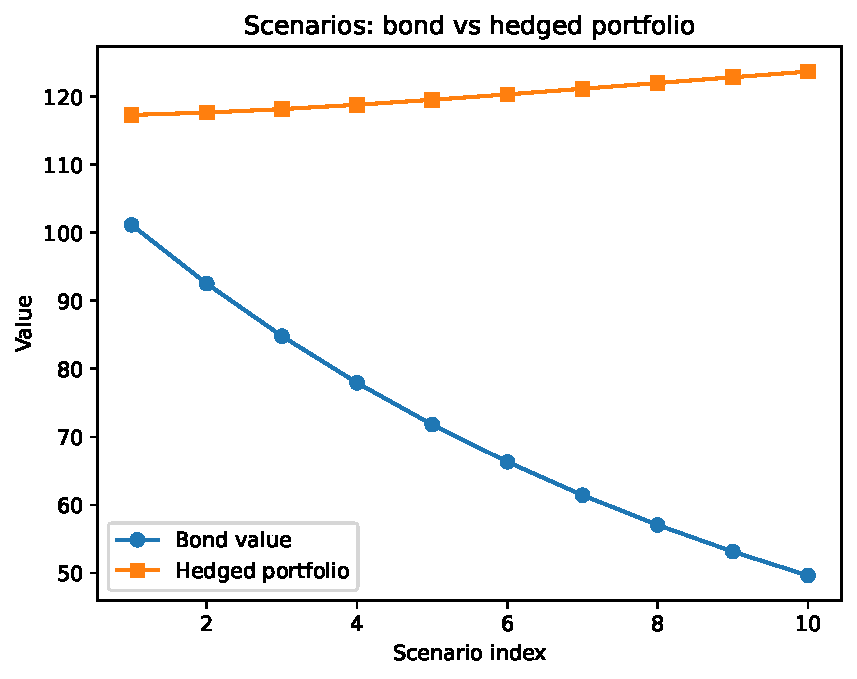
\includegraphics[width=.5\textwidth]{./figures/ECO491_HW5_Q1_Model_1.pdf}
  \caption{Historical Simulation VaR Bond}
\end{figure}

The unhedged bond declines sharply as level and curvature rise, while the hedged portfolio exhibits much smaller changes. The hedge removes first-order exposure to level and curvature; the residual variation reflects higher-order effects.
\section{Bond convexity}
A generic bond with cash flows $\{(\text{CF}_k,T_k)\}_{k=1}^n$ has price
$
P=\sum_{k=1}^n \text{CF}_k e^{-R(T_k)T_k}.
$
A parallel shift changes $R(T_k)\to R(T_k)+dR$ for all $k$ and
\[
\frac{\partial}{\partial R}e^{-RT_k}=-T_k e^{-RT_k},\qquad
\frac{\partial^2}{\partial R^2}e^{-RT_k}=T_k^2 e^{-RT_k},
\]
giving:
\[
\frac{\partial P}{\partial R}
=\sum_{k=1}^n -\text{CF}_k T_k e^{-R(T_k)T_k},\qquad
\frac{\partial^2 P}{\partial R^2}
=\sum_{k=1}^n \text{CF}_k T_k^2 e^{-R(T_k)T_k}.
\]

Traditional duration and convexity:
\[
D=\frac{1}{P}\sum_{k=1}^n \text{CF}_k T_k e^{-R(T_k)T_k},\qquad
C=\frac{1}{P}\sum_{k=1}^n \text{CF}_k T_k^2 e^{-R(T_k)T_k}.
\]

For the 8-year bond:
\begin{center}
\begin{tabular}{c c c c}
$k$ & $T_k$ & $T_k^2$ & $\text{CF}_k e^{-R(T_k)T_k}$ \\ \hline
1  & 0.5 & 0.25 & 2.934 \\
8  & 4.0 & 16.00 & 2.426 \\
12 & 6.0 & 36.00 & 2.281 \\
16 & 8.0 & 64.00 & 84.998 \\
\end{tabular}
\end{center}
$$
\boxed{D=\frac{1}{110.858}\sum_{k=1}^{16}\text{CF}_k T_k e^{-R(T_k)T_k}}
\quad
\boxed{C=\frac{1}{110.858}\sum_{k=1}^{16}\text{CF}_k T_k^2 e^{-R(T_k)T_k}}
$$

Under the polynomial term structure:
\[
R(T)=\beta_1\cdot1+\beta_2 T+\beta_3 T^2,\qquad
f_{\text{lev}}(T)=1,\ f_{\text{slope}}(T)=T,\ f_{\text{curv}}(T)=T^2,
\]
while the price remains
$
P=\sum_{k=1}^n \text{CF}_k e^{-R(T_k)T_k}.
$

Differentiating with respect to factor $\beta_j$:
\[
\frac{\partial P}{\partial\beta_j}
=\sum_{k=1}^n \text{CF}_k(-T_k f_j(T_k))e^{-R(T_k)T_k},\qquad
\frac{\partial^2 P}{\partial\beta_j^2}
=\sum_{k=1}^n \text{CF}_k(T_k f_j(T_k))^2 e^{-R(T_k)T_k}.
\]

Then factor convexity is 
$
C_j=\frac{1}{P}\sum_{k=1}^n (T_k f_j(T_k))^2 \,\text{CF}_k e^{-R(T_k)T_k}.
$

After, one applies the three factor loadings:

\begin{center}
\begin{tabular}{c c}
Factor & Convexity Expression \\ \hline
Level      & $\displaystyle C_{\text{lev}}=\frac{1}{P}\sum CF_k T_k^2 e^{-R(T_k)T_k}$ \\[4pt]
Slope      & $\displaystyle C_{\text{slope}}=\frac{1}{P}\sum CF_k T_k^4 e^{-R(T_k)T_k}$ \\[4pt]
Curvature  & $\displaystyle C_{\text{curv}}=\frac{1}{P}\sum CF_k T_k^6 e^{-R(T_k)T_k}$ \\
\end{tabular}
\end{center}

\section{Black--Scholes option pricing via risk-neutral valuation}

Let the underlying price at time $t$ be $S_t$ and maturity be $T$ and not that the log-return
$
x^*=\ln\!\Big(\frac{S_{t+T}}{S_t}\Big)
$
is normal such that:
$
x^*\sim \mathcal{N}(\mu,\sigma_x^2),\qquad
\mu=T\Big(r_f-\tfrac{1}{2}\sigma^2\Big),\quad
\sigma_x^2=T\sigma^2.
$

The call price with strike $X$ is:
\[
c_t=e^{-r_fT}\,\mathbb{E}^{\mathbb{Q}}\!\big[(S_{t+T}-X)^+\big]
     =e^{-r_fT}\int_{-\infty}^{\infty}\max(S_t e^{x^*}-X,0)\,f(x^*)\,dx^*,
\]
where $f$ is the $\mathcal{N}(\mu,\sigma_x^2)$ density. The payoff is zero when $S_t e^{x^*}\le X$, i.e.\ when
$
x^*\le k \text{ and } k=\ln\!\Big(\frac{X}{S_t}\Big),
$
so the integral starts at $k$:
\[
c_t=e^{-r_fT}\int_{k}^{\infty}(S_t e^{x^*}-X)\,f(x^*)\,dx^*
   =e^{-r_fT}\Big[
     S_t\int_{k}^{\infty}e^{x^*}f(x^*)\,dx^*
    -X\int_{k}^{\infty}f(x^*)\,dx^*
   \Big].
\]

Standardize $x^*$ via
$
z=\frac{x^*-\mu}{\sigma_x} \text{ and } x^*=\mu+\sigma_x z,
$
and let $\varphi$ and $\Phi$ be the standard normal pdf and cdf. Then follow the following computations:
\[
\int_{k}^{\infty}f(x^*)\,dx^*=\Phi(d_2),
\qquad
d_2=\frac{\ln(S_t/X)+(r_f-\tfrac{1}{2}\sigma^2)T}{\sigma\sqrt{T}},
\]
\[
\int_{k}^{\infty}e^{x^*}f(x^*)\,dx^*
=e^{\mu+\tfrac{1}{2}\sigma_x^2}\Phi(d_1)
=e^{r_fT}\Phi(d_1),
\]
\[
d_1=\frac{\ln(S_t/X)+(r_f+\tfrac{1}{2}\sigma^2)T}{\sigma\sqrt{T}},
\qquad d_2=d_1-\sigma\sqrt{T}.
\]

Substitute into the pricing integral:
\[
c_t=e^{-r_fT}\Big[S_t e^{r_fT}\Phi(d_1)-X\Phi(d_2)\Big]
    =S_t\Phi(d_1)-X e^{-r_fT}\Phi(d_2).
\]

Thus the Black--Scholes call price and $d_1,d_2$ are
\[
\boxed{c_t=S_t\Phi(d_1)-X e^{-r_fT}\Phi(d_2)}
\]
\[
\boxed{
d_1=\frac{\ln(S_t/X)+(r_f+\tfrac{1}{2}\sigma^2)T}{\sigma\sqrt{T}},
\quad
d_2=d_1-\sigma\sqrt{T}
}
\]

\section{Black--Scholes delta}

Consider a European call (no dividends) with price
$
c_t(S_t)=S_t\Phi(d_1)-K e^{-r_f T}\Phi(d_2),
$
where:
\[
d_1=\frac{\ln(S_t/K)+(r_f+\tfrac{1}{2}\sigma^2)T}{\sigma\sqrt{T}},\qquad
d_2=d_1-\sigma\sqrt{T}.
\]

\subsection*{4.1 \quad Delta of a call}

Delta is
$
\delta=\frac{\partial c_t}{\partial S_t}
$
so differentiate
$
\frac{\partial c_t}{\partial S_t}
=\Phi(d_1)+S_t\varphi(d_1)\frac{\partial d_1}{\partial S_t}
   -K e^{-r_f T}\varphi(d_2)\frac{\partial d_2}{\partial S_t}.
$
using
$
\frac{\partial d_1}{\partial S_t}=\frac{1}{S_t\sigma\sqrt{T}} \text{ and }
\frac{\partial d_2}{\partial S_t}=\frac{\partial d_1}{\partial S_t},
$
and the identity
$
S_t\varphi(d_1)=K e^{-r_f T}\varphi(d_2).
$
\\ \\
The terms with $\varphi$ cancel and finally we are left with:
$
\boxed{\delta=\Phi(d_1)}.
$
Thus the Black--Scholes call delta equals the risk-neutral probability that the option finishes in the money.

\subsection*{4.2 \quad Delta as a function of the underlying price}

\begin{figure}[H]
  \centering
  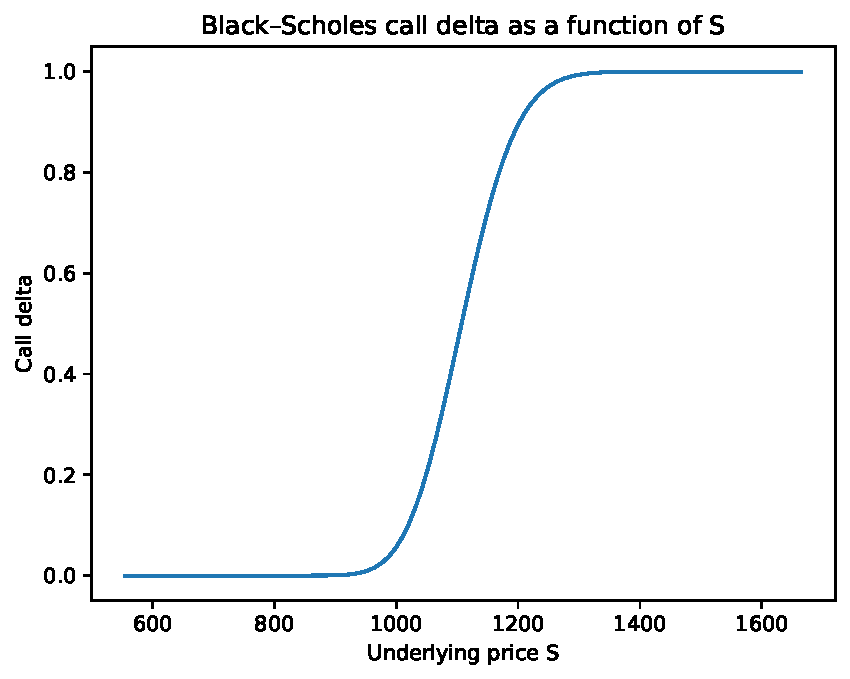
\includegraphics[width=.5\textwidth]{./figures/ECO491_HW5_Q4_Model_1.pdf}
  \caption{Historical Simulation VaR Bond}
\end{figure}

Fix $(K,T,r_f,\sigma)$ and view
$
\delta(S_t)=\Phi\!\left(
\frac{\ln(S_t/K)+(r_f+\tfrac{1}{2}\sigma^2)T}{\sigma\sqrt{T}}
\right)
$
as a function of $S_t$ (or moneyness $S_t/K$). Delta is an increasing S-shaped curve:
\[
\delta(S_t)\to 0 \text{ as } S_t\to 0,\qquad
\delta(S_t)\to 1 \text{ as } S_t\to\infty.
\]

For the S\&P 500 example in the lecture
$
K=1110,\quad T=\frac{43}{365},\quad r_f=0.0025,\quad \sigma=0.1872,
$
the graph of $\delta(S_t)$ against $S_t$ has a steep region near $S_t\approx K$ and flattens out deep in- or out-of-the-money. Around the steep middle region, small changes in $S_t$ produce large changes in $\delta$, so the linear approximation
$
\Delta c\approx \delta\,\Delta S
$
is less accurate; in the flatter tails delta is nearly constant and the linear approximation is much more accurate.

\section{Black--Scholes implied volatility and monotonicity}
\subsection*{5.1 \quad Call price is increasing in volatility}

For a non-dividend-paying stock the Black--Scholes call price is
\[
c_{\text{BS}}(S,r_f,K,T,\sigma)
=S\Phi(d_1)-K e^{-r_fT}\Phi(d_2),
\]
where
\[
d_1=\frac{\ln(S/K)+(r_f+\tfrac{1}{2}\sigma^2)T}{\sigma\sqrt{T}},
\qquad
d_2=d_1-\sigma\sqrt{T}.
\]

The derivative w.r.t.\ $\sigma$ (vega) is
$
\frac{\partial c_{\text{BS}}}{\partial\sigma}
=S\varphi(d_1)\sqrt{T}.
$
Since $S>0$, $\sqrt{T}>0$ and $\varphi(d_1)>0$ for all real $d_1$ then it follows that
$\boxed{\frac{\partial c_{\text{BS}}}{\partial\sigma}>0}
$
such that the Black--Scholes call price is strictly increasing in volatility.

\subsection*{5.2 \quad Put price is increasing in volatility}

Put–call parity (no dividends) gives
$
c_{\text{BS}}(S,r_f,K,T,\sigma)-p_{\text{BS}}(S,r_f,K,T,\sigma)
=S-K e^{-r_fT},
$
which does not depend on $\sigma$. Differentiate w.r.t.\ $\sigma$:
\[
\frac{\partial c_{\text{BS}}}{\partial\sigma}
-\frac{\partial p_{\text{BS}}}{\partial\sigma}=0
\quad\Rightarrow\quad
\frac{\partial p_{\text{BS}}}{\partial\sigma}
=\frac{\partial c_{\text{BS}}}{\partial\sigma}
=S\varphi(d_1)\sqrt{T}.
\]
Then $S>0$, $\sqrt{T}>0$, $\varphi(d_1)>0$ such that it follows immediately that
$
\boxed{\frac{\partial p_{\text{BS}}}{\partial\sigma}>0}
$
so the Black--Scholes put price is also strictly increasing in volatility.
